\section{Method}
\label{sec:method}

\subsection{Data}
\label{sec:data}

This study focuses on stellar rotation in the original \kepler\ field.
This is partly because \kepler\ provides the largest sample of published,
homogeneously measured rotation periods, and partly because its low Galactic
latitude allows us to more easily marginalize over missing RV measurements and
approximate vertical velocity, \vz.

We combined two large rotation period catalogs constructed from original
\kepler\ data, from \citet{mcquillan2014} and \citet{santos2019}.
These two studies used different techniques to measure rotation periods from
\kepler\ light curves: autocorrelation functions and wavelets respectively.
The \citet{santos2019} study was specifically focused on cooler stars: K and M
dwarfs, and includes a larger number of rotation periods for these stars.
The combined catalogs provide a total of over 38,000 rotation periods.

To calculate kinematic ages, an estimate of vertical velocity, \vz, is
required.
The ideal way to calculated \vz\, and similarly, \vx\ and \vy, is to use 6D
positional and velocity information.
Many stars in the \kepler\ field do not have RV measurements and an
alternative approach must be taken to infer their vertical velocities (see
section \ref{sec:velocity_inference}).
However, a large number of \kepler\ rotators, over 10,000 of 34,000 {\it do}
have RV measurements from \gaia\ DR2 and \lamost.
Figure \ref{fig:existing_rvs} shows rotation period vs effective temperature
for all stars in the \mct\ and \citet{santos2019} catalogs, plotted in grey.
Stars with RV measurements are colored by their vertical velocity dispersion
(see section \ref{sec:velocity_dispersion} to see how we calculated velocity
dispersion).
\racomment{Discuss what this plot shows}.

Although RVs are available for a significant number of \kepler\ rotators
(almost one in three), few stars cooler than 4000 K have RV measurements.
This is due to the faint limits of the \gaia\ DR2 and \lamost\ surveys
(although RV measurements for fainter targets will be available in \gaia\
DR3).
Given that magneto-rotational evolution is poorly understood for M dwarfs, the
cool stars with missing RVs are arguably the ones we care most about.
For this reason, we attempt to compensate for the lack of RV measurements by
inferring vertical velocities for stars without RVs, filling in the
low-temperature region of figure \ref{fig:existing_rvs} in section
\ref{sec:velocity_inference}.
\begin{figure}[ht!]
\caption{
Vertical velocity dispersion as a function of rotation period and effective
    temperature for \kepler\ stars with measured rotation periods.
Colored points show stars with RV measurements from \gaia\ or \lamost, with
    their color indicating their velocity dispersion.
Faint grey points show the combined \mct\ and \citet{santos2019} samples,
    including stars without RV measurements.
The coolest stars in this sample do not have RVs because they are faint.
}
  \centering 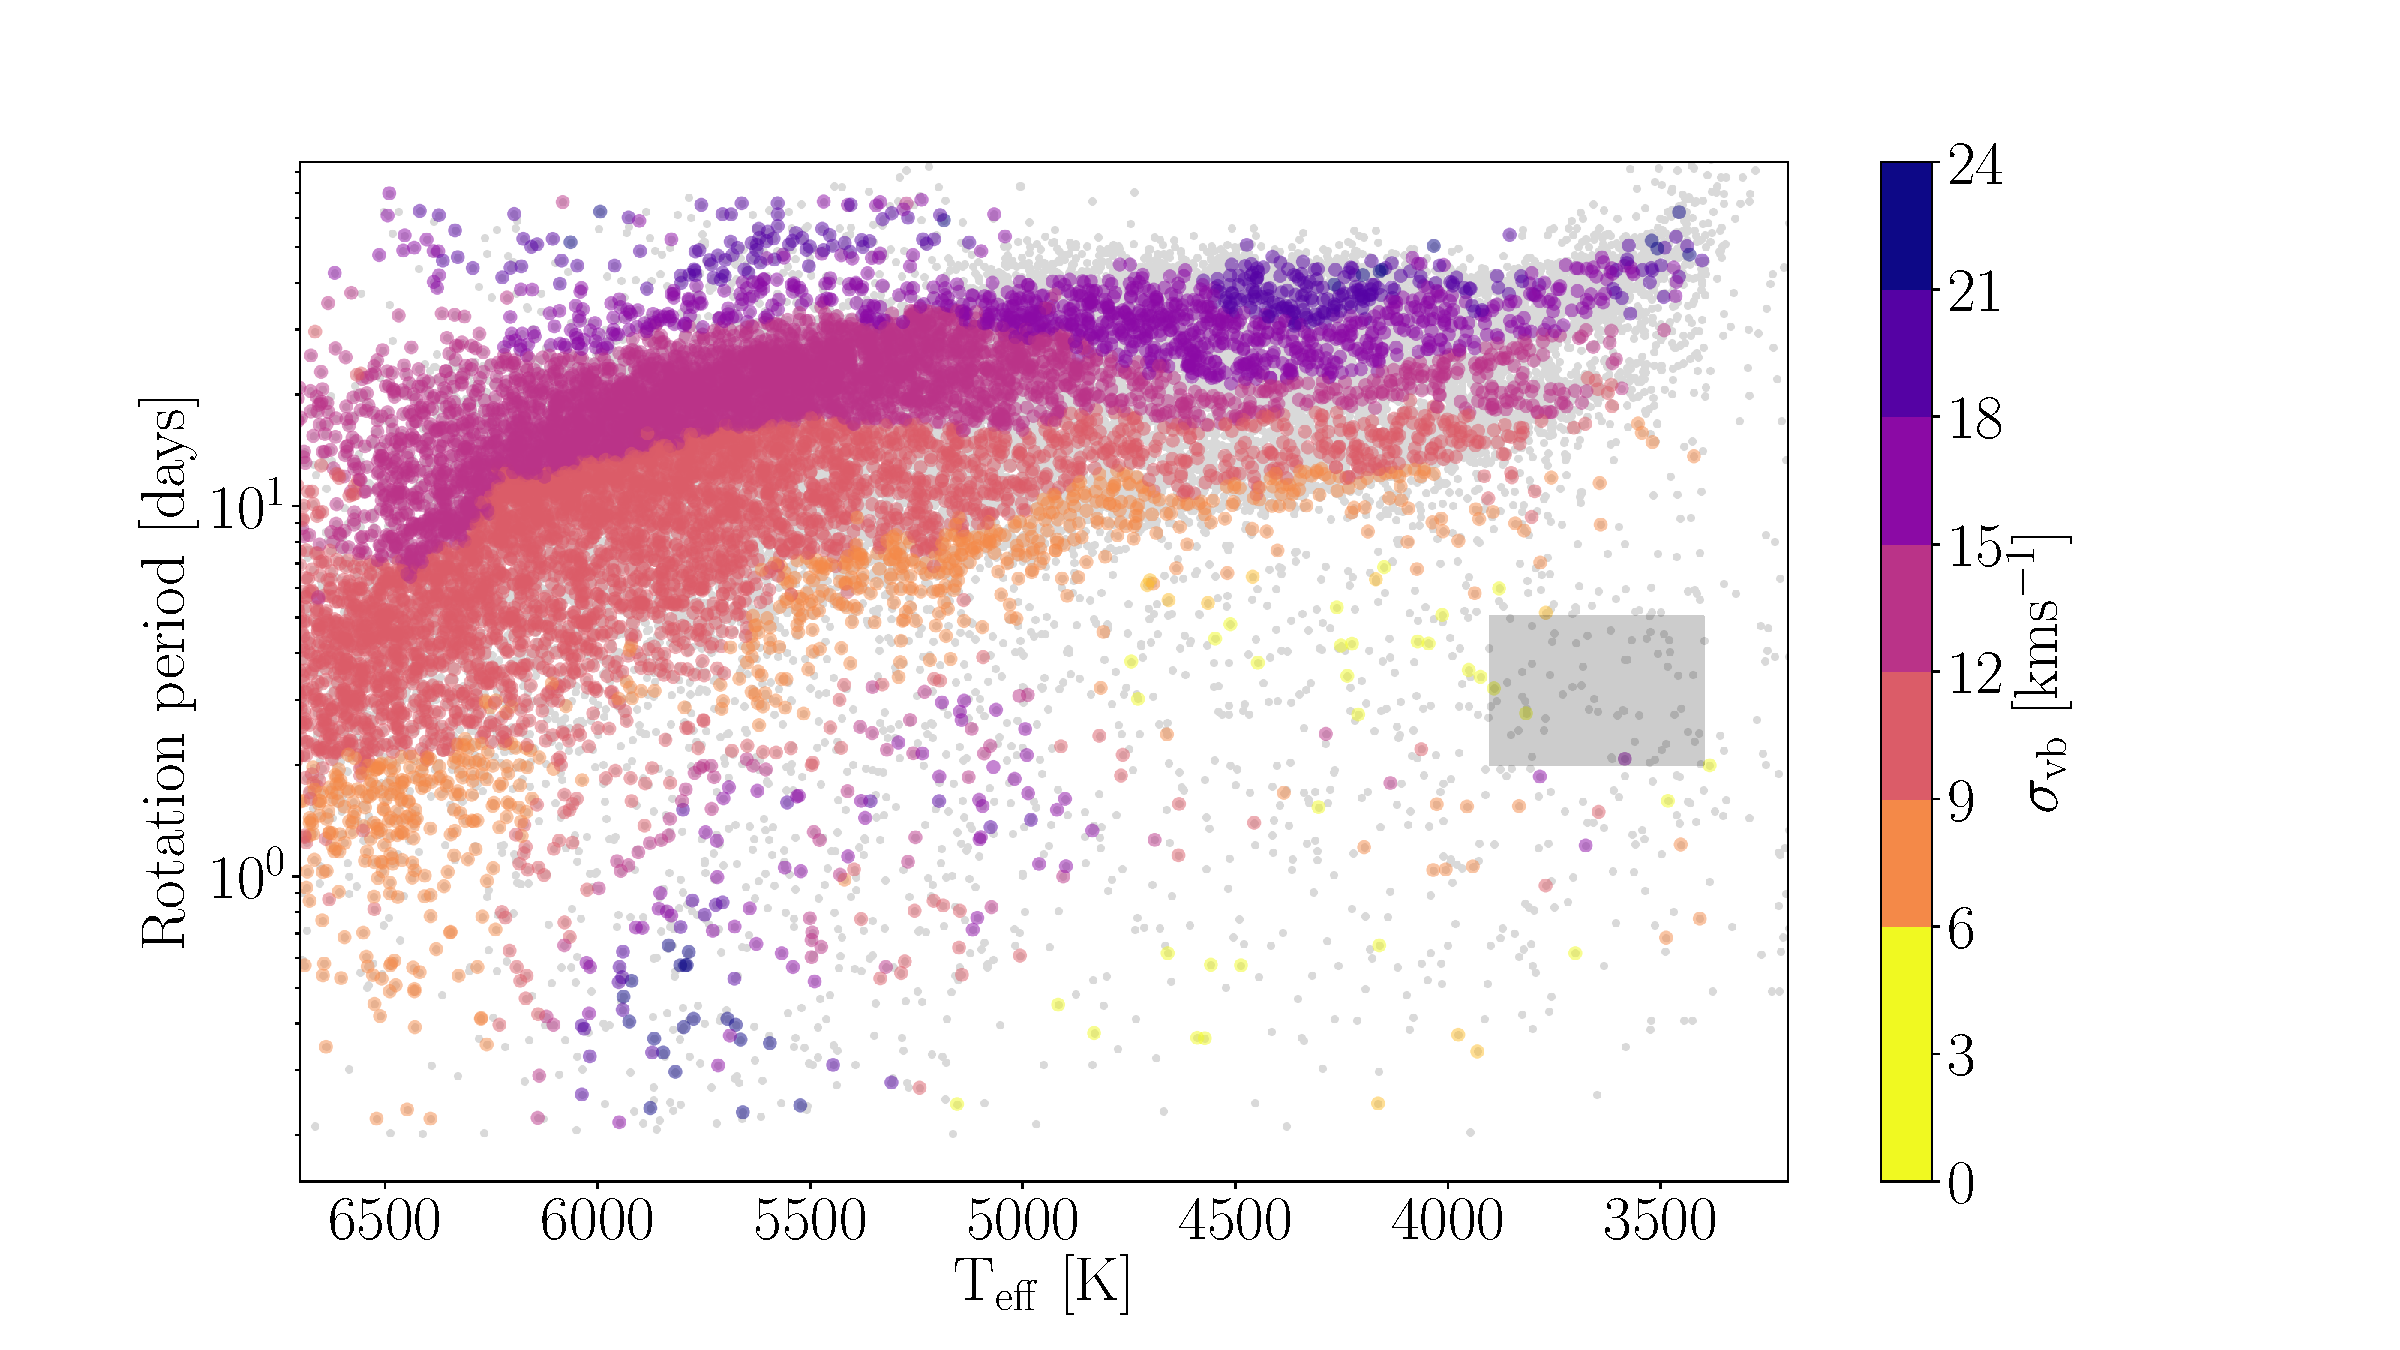
\includegraphics[width=1\textwidth]{existing_rvs}
\label{fig:existing_rvs}
\end{figure}


\subsection{Inferring 3D velocities (marginalizing over missing RV
measurements)}
\label{sec:velocity_inference}

It has been demonstrated that the dispersion in vertical velocity, \vz\, for a
group of stars increases with the age of that group (citations).
However, velocities in Galactocentric coordinates, \vx, \vy\ and \vz, can only
be calculated with full 6-D position and velocity information, \ie\ proper
motions, position and radial velocity.
In Angus \etal\ (2020) we introduced the idea that kinematic ages could be
used to calibrate gyrochronology and showed, in the appendix of that paper,
that velocity, \vb\ in the Galactic frame, which can be calculated without an
RV measurement, can be used as an approximation to \vz\ for \kepler\ stars.
This is because the \kepler\ field of view lies at relatively low Galactic
latitudes, ($\sim 5-20$\degrees), so the $z$-direction is similar to the
$b$-direction for \kepler\ stars.
However, \vb\ is only a close approximation to \vz\ at extremely {\it low}
latitudes, and even in the \kepler\ field, kinematic ages calculated with \vb\
instead of \vz\ are systematically larger because of extra noise introduced by
the imperfect translation between \vb\ and \vz\.
In order to calculate accurate vertical velocities and therefore ages, the
appropriate approach is to {\it infer} \vz\  by marginalizing over missing RV
measurements.

% Three-dimensional velocities in galactocentric coordinates: \vx, \vy, and \vz\
% can only be directly computed via a transformation from 3D velocities in
% another coordinate system, like the equatorial coordinates provided by \gaia:
% \mura, \mudec, and RV.
% For stars with no measured RV in \gaia\ DR2, \vx, vy, and \vz\ can still be
% inferred from positions and proper motions alone, by marginalizing over
% missing RV measurements.
For each star in our sample, we inferred \vx, \vy, and \vz\ from the 3D
positions and proper motions provided in the \gaia\ DR2 catalog
\citep{brown2011}.
We also simultaneously inferred distance, instead of using 1/\parallax, to
model velocities \citep{bailer-jones2015, bailer-jones2018}.

Using Bayes rule, the posterior probability of the parameters given the data
can be written:
\begin{equation}
p(v_{\bf xyz}, D | \mu_{\alpha}, \mu_{\delta}, \alpha, \delta, \pi) =
    p(\mu_{\alpha}, \mu_{\delta}, \alpha, \delta, \pi | v_{\bf xyz}, D)
    p(v_{\bf xyz}) p(D),
\end{equation}
where D is distance, $\alpha$ is Right Ascension (RA), $\delta$ is declination
(dec), $\pi$ is parallax, $\mu_\alpha$ is proper motion in RA, and
$\mu_\delta$ is proper motion in dec.
The prior over $\log$(distance) and velocities was a multivariate Gaussian
with mean and covariance determined from the distance and velocity
distributions of \kepler\ targets with RV measurements.

The posterior PDF was explored using {\tt emcee} \citep{foreman-mackey2013},
an affine-invariant, ensemble MCMC sampler.

Initialization.

We found that 10,000 samples with 16 walkers was sufficient to calculate a
converged autocorrelation time, and produce 150-500 independent samples per
parameter.

Over 3000 stars in the \mct\ sample do have RV measurements and provide an
opportunity to test this method of inferring velocities.
Figure \ref{fig:v_comparison} shows the velocities of these 3000 stars,
calculated using RV measurements, compared with their inferred velocities.
\begin{figure}[ht!]
\caption{Vertical velocities calculated with full 6D information vs vertical
    velocities inferred without RV, for all 3000 \mct\ stars with \gaia\ RV
    measurements.}
  \centering
    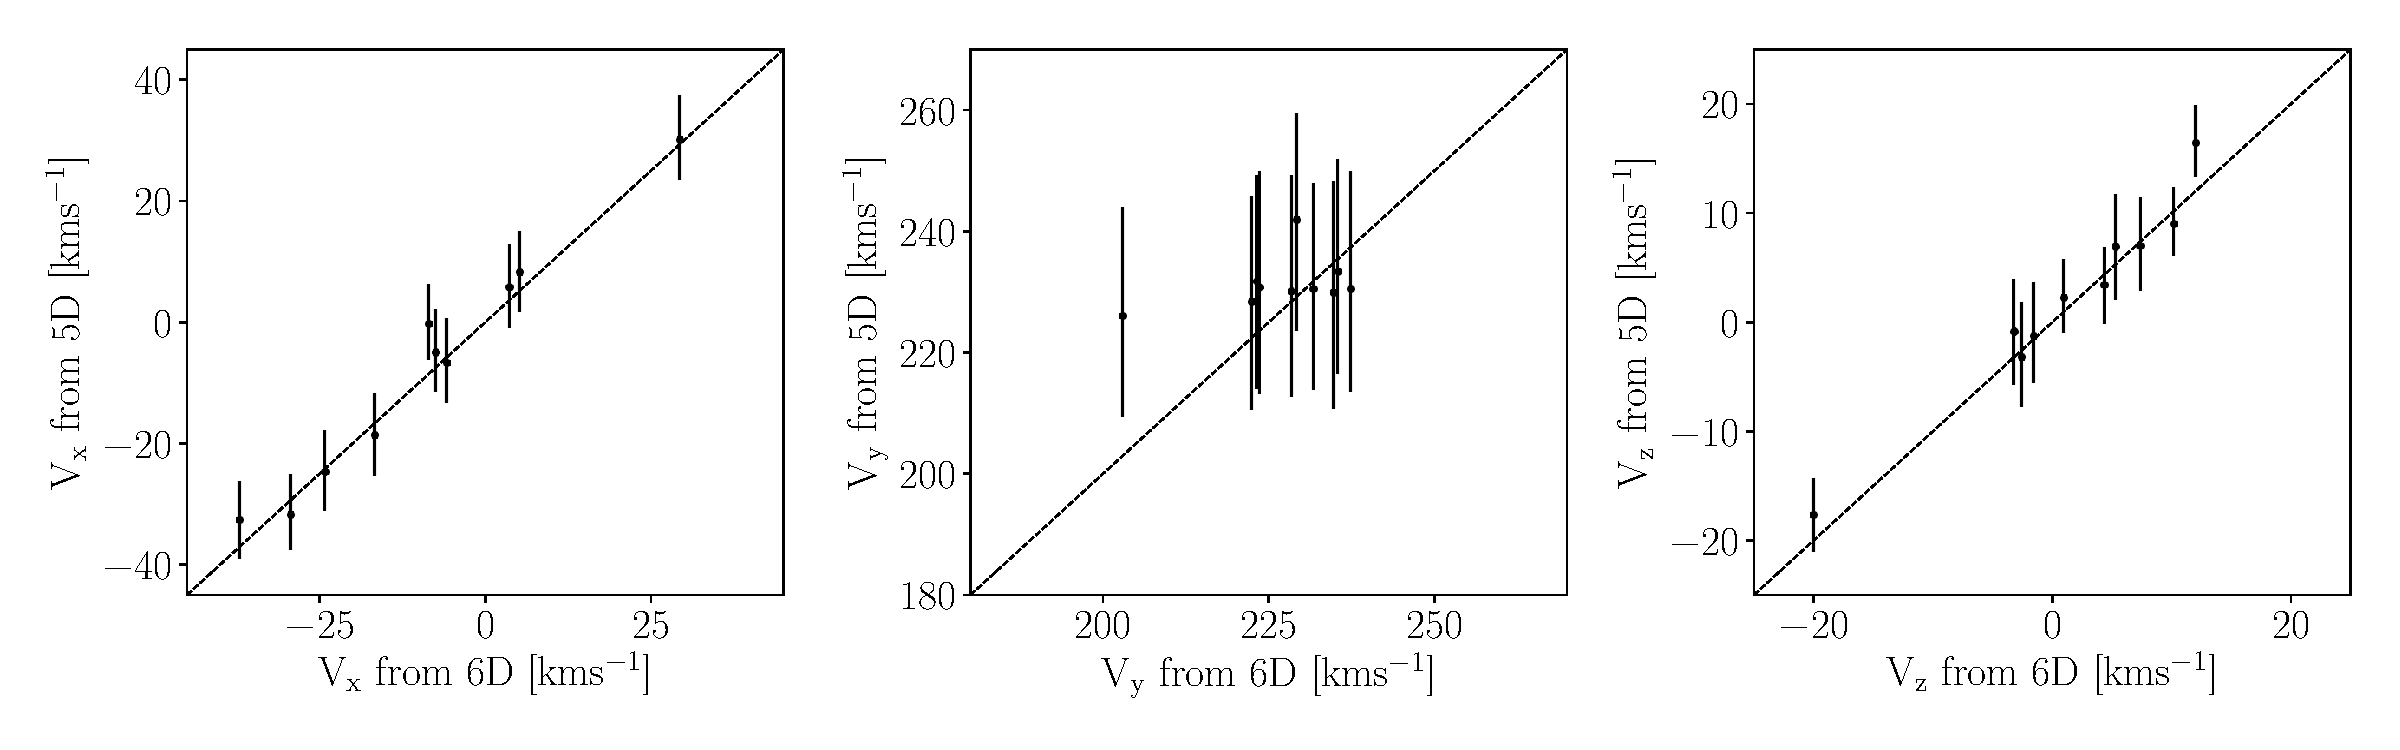
\includegraphics[width=1\textwidth]{v_comparison}
\label{fig:v_comparison}
\end{figure}

\subsection{Calculating velocity dispersions}
\label{sec:velocity_dispersion}

A kinematic age can be calculated from the velocity dispersion of a group of
stars (where `dispersion' is usually the standard deviation of velocities).
These velocity dispersions can then be converted into an age using an AVR
\citep[\eg][]{holmberg2009, yu2018}.
The major assumption underlying kinematic ages is that all stars used to
calculate a velocity dispersion are {\it the same age}.
So, in order to calculate kinematic ages from velocity dispersions for
\kepler\ stars, it is necessary to group them by age.
Fortunately, we can use the implicit assumption that underpins gyrochronology
itself to group stars by age: that stars with the same rotation period and
color are the same age.
We discuss the implications of this assumption, and how our results would
change if this assumption is false, in the Discussion of this paper (section
\ref{sec:discussion}).

To calculate a \vz\ velocity dispersion and therefore age for each \kepler\
star, we grouped stars with their neighbors in
\logp--\teff\ space.
We experimented with two methods of grouping stars: using K-nearest neighbors,
and using a fixed range in \logp\ and \teff.
In the K-nearest neighbors method, each star was grouped with the K-nearest
stars in \logp-\teff\ space.
Groups created this way span a small range of \logp\ and \teff\ where the
number density of stars is large, and a large range where the number density
is small.
However, all groups have the same number of stars.
In the fixed range method, each star was grouped with stars whose \logp s and
\teff s fell within a certain range of their own.
This method created groups with large numbers of stars in densely populated
regions of the \logp--\teff\ plane, and small numbers of stars in sparsely
populated regions, \ie\ each group contains a different number of stars.
However, the bin size was constant.
To choose the best method, and to optimize for the parameters of each (K and
\logp\ and \teff-range), we conducted a set of tests.


\subsection{Converting velocity dispersion to age with an AVR}
\label{sec:avr}

\subsection{Comparing kinematic ages with asteroseismic and cluster ages}

\subsection{A Gaussian process gyrochronology relation}
\label{sec:gp_model}
